% author: Tomas Trnka
% mail: tomas@trnkatomas.eu
% date: 2013-07-04

\documentclass[a4paper,10pt]{article}
%\usepackage[czech]{babel}
%\usepackage[T1]{fontenc}
\usepackage[hmargin=2.2cm,vmargin=2.2cm]{geometry}
\usepackage[utf8x]{inputenc}
\usepackage{fancyhdr}
\usepackage{amsmath} 
\usepackage{tikz}
\usetikzlibrary{patterns}
\usepackage{enumerate}
\pagestyle{fancy}
\headheight 15pt
\lhead{Crpyto, Fall 2014}
\rhead{Tomas Trnka}
\def\firstcircle{(270:1.75cm) circle (2.5cm)}
\def\secondcircle{(150:1.75cm) circle (2.5cm)}
\def\thirdcircle{(30:1.75cm) circle (2.5cm)}
\begin{document}
\section*{Entropies}
\begin{enumerate}[a)]
\item I~decided to solve the task with help of venn diagrams.

\begin{figure}[h!]
\centering
 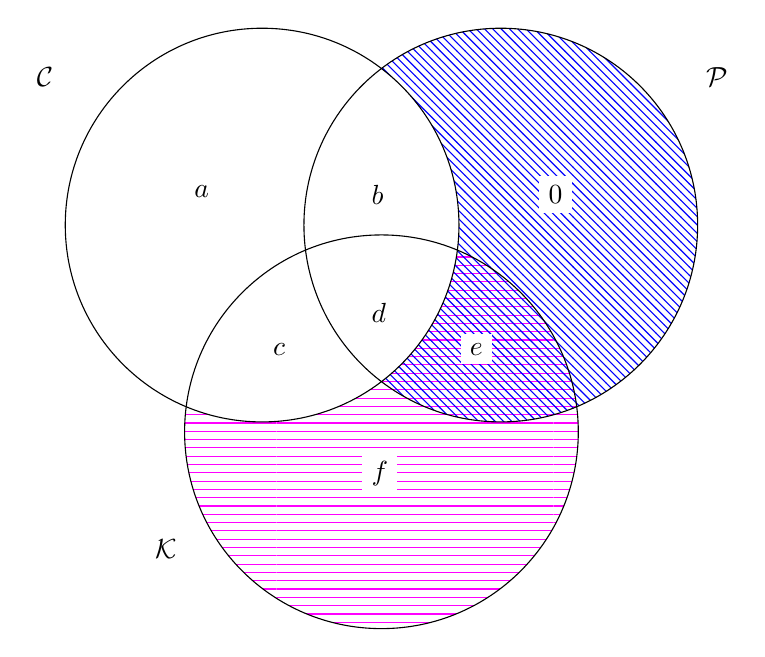
\begin{tikzpicture}
   \begin{scope}
    	\clip \firstcircle;
	    \fill[pattern=horizontal lines, pattern color=magenta,even odd rule] \secondcircle \firstcircle;     	%cyan,opacity=0.2
   \end{scope}
   \begin{scope}
    	\clip \thirdcircle;
	    \fill[pattern=north west lines, pattern color=blue, even odd rule] \secondcircle \thirdcircle;
   \end{scope}
      \draw \firstcircle node[text=black,above] {};
      \draw \secondcircle node [text=black,below left] {};
      \draw \thirdcircle node [text=black,below right] {};
      \draw node at (4,3) [text=black,below right] {$\mathcal{P}$};
      \draw node at (-3,-3) [text=black,below right] {$\mathcal{K}$};
      \draw node at (-4.5,3) [text=black,below right] {$\mathcal{C}$};
      \draw node at (-2.5,1.5) [text=black,below right] {$a$};
      \draw node[fill=white] at (2,1.5) [text=black,below right] {$0$};
      \draw node[fill=white] at (-0.25,1.5) [text=black,below right] {$b$};
      \draw node[fill=white] at (-1.5,-0.5) [text=black,below right] {$c$};
      \draw node[fill=white] at (-0.25,0) [text=black,below right] {$d$};
      \draw node[fill=white] at (1,-0.5) [text=black,below right] {$e$};
      \draw node[fill=white] at (-0.25,-2) [text=black,below right] {$f$};
    \end{tikzpicture}    
\end{figure}

From the picture we can see that the entropy $ H(P|C) = e + 0 $. The other entropy $H(K|C)$ is equal to $e+f$. The symbol $f$ stands for entropy $H(K|C,P)$ and as we know entropy is always greater or equal to zero. From this we can simply substitute and obtain the result:
\begin{eqnarray*}
e &=& e\\
e + 0 &\leq & e + f\\
H(P|C) &\leq & H(K|C)
\end{eqnarray*}
Therefore we can say that the we have proven that the equation is correct.


\item The second task is to answer the question when holds true that $H(K|C) = H(P|C)$. To fulfil this equality it is necessary for $f$ to be zero (we can conclude this from the equations above). This means that $H(K|P,C)=0$ that can be "translated" as when we know both cipher and plain text  we can say what the key is. This is true for rather simple ciphers like for example simple shift ciphers such as Caesar cipher of affine cipher.
\end{enumerate}
\end{document}